% Options for packages loaded elsewhere
\PassOptionsToPackage{unicode}{hyperref}
\PassOptionsToPackage{hyphens}{url}
%
\documentclass[
  ignorenonframetext,
]{beamer}
\usepackage{pgfpages}
\setbeamertemplate{caption}[numbered]
\setbeamertemplate{caption label separator}{: }
\setbeamercolor{caption name}{fg=normal text.fg}
\beamertemplatenavigationsymbolsempty
% Prevent slide breaks in the middle of a paragraph
\widowpenalties 1 10000
\raggedbottom
\setbeamertemplate{part page}{
  \centering
  \begin{beamercolorbox}[sep=16pt,center]{part title}
    \usebeamerfont{part title}\insertpart\par
  \end{beamercolorbox}
}
\setbeamertemplate{section page}{
  \centering
  \begin{beamercolorbox}[sep=12pt,center]{part title}
    \usebeamerfont{section title}\insertsection\par
  \end{beamercolorbox}
}
\setbeamertemplate{subsection page}{
  \centering
  \begin{beamercolorbox}[sep=8pt,center]{part title}
    \usebeamerfont{subsection title}\insertsubsection\par
  \end{beamercolorbox}
}
\AtBeginPart{
  \frame{\partpage}
}
\AtBeginSection{
  \ifbibliography
  \else
    \frame{\sectionpage}
  \fi
}
\AtBeginSubsection{
  \frame{\subsectionpage}
}
\usepackage{amsmath,amssymb}
\usepackage{iftex}
\ifPDFTeX
  \usepackage[T1]{fontenc}
  \usepackage[utf8]{inputenc}
  \usepackage{textcomp} % provide euro and other symbols
\else % if luatex or xetex
  \usepackage{unicode-math} % this also loads fontspec
  \defaultfontfeatures{Scale=MatchLowercase}
  \defaultfontfeatures[\rmfamily]{Ligatures=TeX,Scale=1}
\fi
\usepackage{lmodern}
\usefonttheme{professionalfonts}
\ifPDFTeX\else
  % xetex/luatex font selection
\fi
% Use upquote if available, for straight quotes in verbatim environments
\IfFileExists{upquote.sty}{\usepackage{upquote}}{}
\IfFileExists{microtype.sty}{% use microtype if available
  \usepackage[]{microtype}
  \UseMicrotypeSet[protrusion]{basicmath} % disable protrusion for tt fonts
}{}
\makeatletter
\@ifundefined{KOMAClassName}{% if non-KOMA class
  \IfFileExists{parskip.sty}{%
    \usepackage{parskip}
  }{% else
    \setlength{\parindent}{0pt}
    \setlength{\parskip}{6pt plus 2pt minus 1pt}}
}{% if KOMA class
  \KOMAoptions{parskip=half}}
\makeatother
\usepackage{xcolor}
\newif\ifbibliography
\usepackage{graphicx}
\makeatletter
\def\maxwidth{\ifdim\Gin@nat@width>\linewidth\linewidth\else\Gin@nat@width\fi}
\def\maxheight{\ifdim\Gin@nat@height>\textheight\textheight\else\Gin@nat@height\fi}
\makeatother
% Scale images if necessary, so that they will not overflow the page
% margins by default, and it is still possible to overwrite the defaults
% using explicit options in \includegraphics[width, height, ...]{}
\setkeys{Gin}{width=\maxwidth,height=\maxheight,keepaspectratio}
% Set default figure placement to htbp
\makeatletter
\def\fps@figure{htbp}
\makeatother
\setlength{\emergencystretch}{3em} % prevent overfull lines
\providecommand{\tightlist}{%
  \setlength{\itemsep}{0pt}\setlength{\parskip}{0pt}}
\setcounter{secnumdepth}{-\maxdimen} % remove section numbering
% \usetheme{metropolis}  
\usepackage{fancyhdr}
\usepackage{lastpage}
\setbeamertemplate{footline}[frame number]{}
\setbeamertemplate{navigation symbols}{}
\pagenumbering{arabic}
% \usepackage[mathbf,mathcal]{euler}
\usepackage{multicol}


\newenvironment{cols}[1][]{}{}

\newenvironment{col}[1]{\begin{minipage}{#1}\ignorespaces}{%
\end{minipage}
\ifhmode\unskip\fi
\aftergroup\useignorespacesandallpars}

\def\useignorespacesandallpars#1\ignorespaces\fi{%
#1\fi\ignorespacesandallpars}

\makeatletter
\def\ignorespacesandallpars{%
  \@ifnextchar\par
    {\expandafter\ignorespacesandallpars\@gobble}%
    {}%
}
\makeatother
\ifLuaTeX
  \usepackage{selnolig}  % disable illegal ligatures
\fi
\IfFileExists{bookmark.sty}{\usepackage{bookmark}}{\usepackage{hyperref}}
\IfFileExists{xurl.sty}{\usepackage{xurl}}{} % add URL line breaks if available
\urlstyle{same}
\hypersetup{
  pdftitle={Mecanismos causales y mediación},
  hidelinks,
  pdfcreator={LaTeX via pandoc}}

\title{Mecanismos causales y mediación}
\author{Diseño e implementación de experimentos en ciencias sociales\\
\emph{Departamento de Economía (UdelaR)}}
\date{}

\begin{document}
\frame{\titlepage}

\begin{frame}{Mecanismos}
\protect\hypertarget{mecanismos}{}
\begin{itemize}
\item
  Queremos describir no sólo la magnitud y el sentido de un efecto
  causal observado, sino también el mecanismo (o mecanismos) que lo
  produjo.
\item
  Qué parde del efecto causal pasa a través de una variable mediadora
\end{itemize}
\end{frame}

\begin{frame}{Estimandos}
\protect\hypertarget{estimandos}{}
Descomponer el efecto total del tratamiento en:

\begin{itemize}
\item
  Efecto indirecto sobre un mediador que luego afecta el resultado,
  llamado efecto de mediación causal promedio (ACME)
\item
  Efecto directo promedio restante (ADE) del tratamiento.
\end{itemize}
\end{frame}

\begin{frame}{Supuesto de ``ignorabilidad secuencial''}
\protect\hypertarget{supuesto-de-ignorabilidad-secuencial}{}
\begin{itemize}
\item
  Sin embargo, una estimación no-sesgada de estos efectos requiere un
  conjunto de supuestos sólidos sobre la relación entre el tratamiento,
  los mediadores, la variable de resultado y los posibles factores de
  confusión.
\item
  colectivamente ignorabilidad secuencial (Imai, Keele y Yamamoto
  (2010), Bullock, Green y Ha (2010)
\end{itemize}
\end{frame}

\begin{frame}{``Sequential ignorability''}
\protect\hypertarget{sequential-ignorability}{}
\center 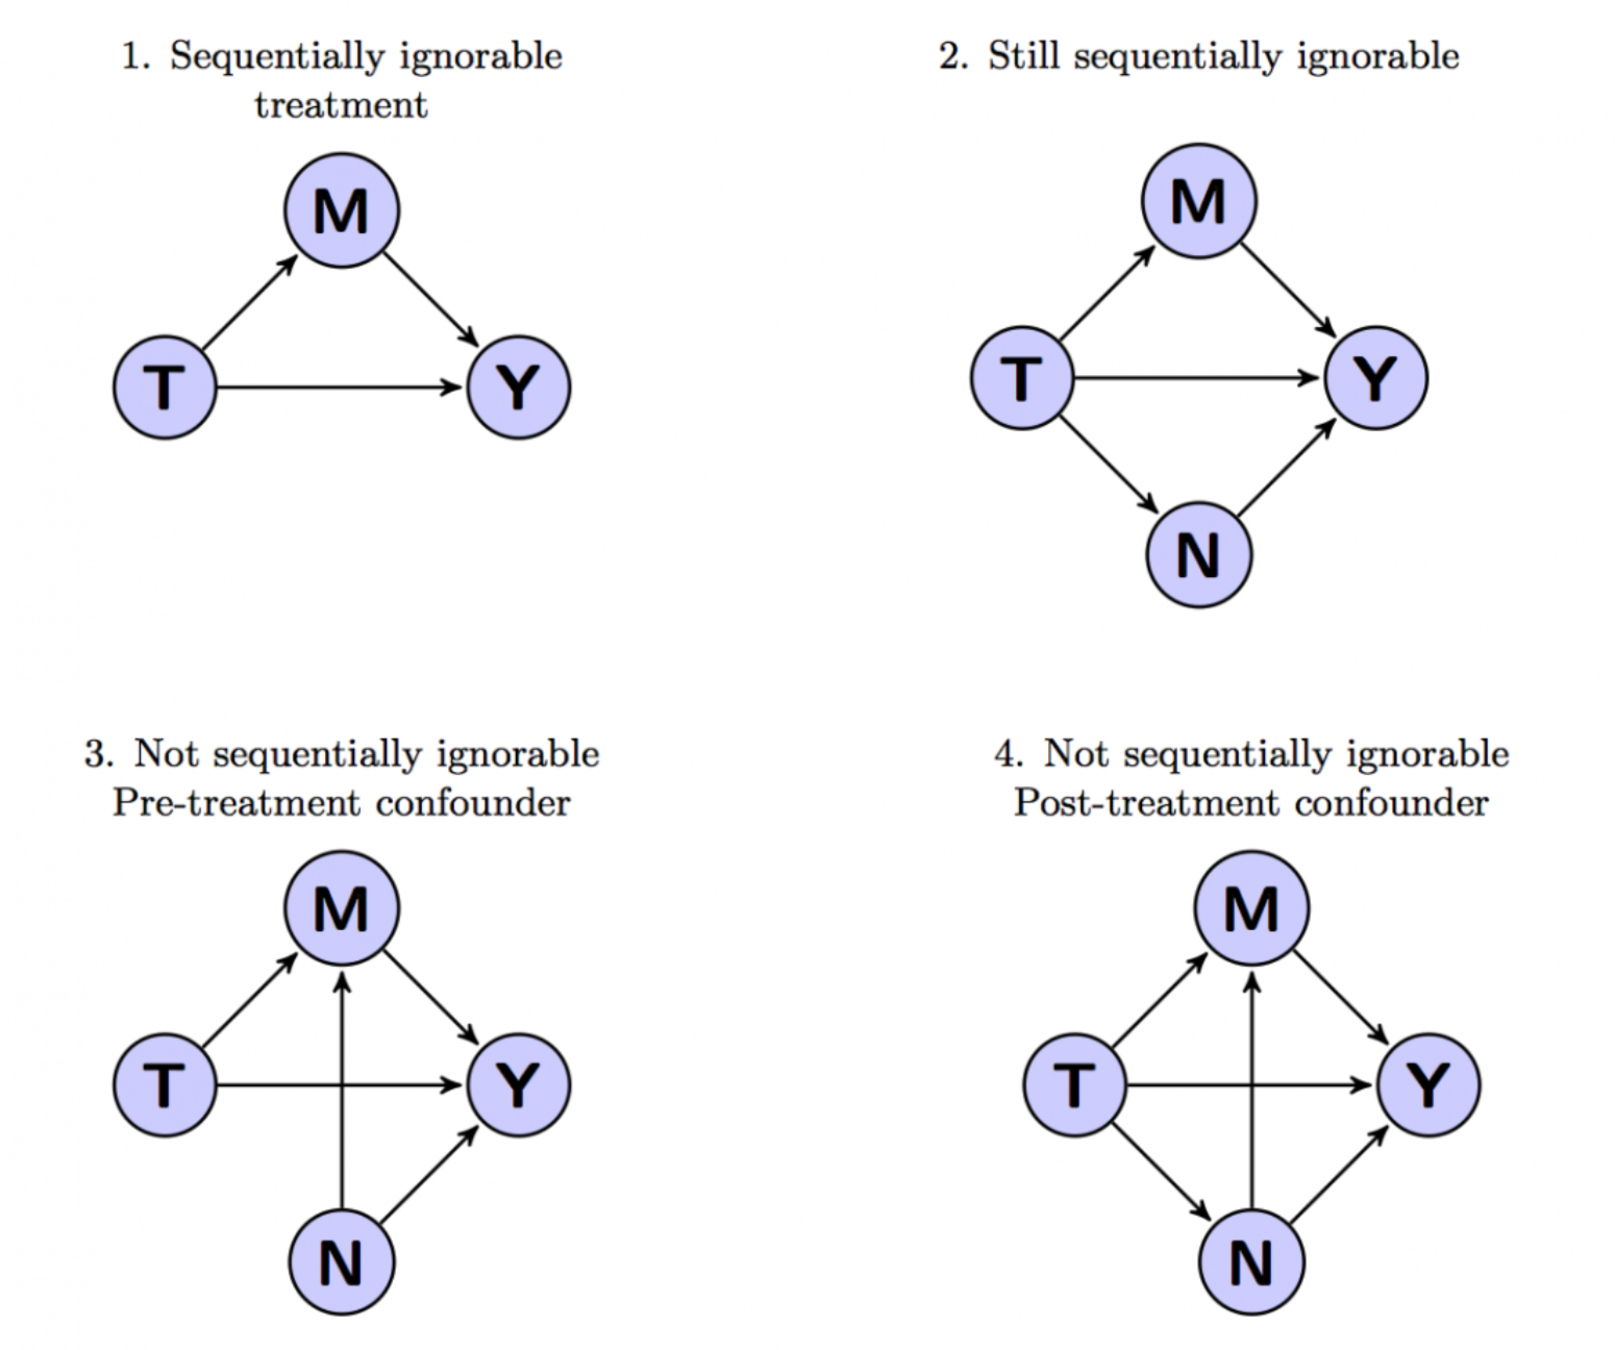
\includegraphics[width=0.8\textwidth,height=\textheight]{figs/sequential_ignorability}
\end{frame}

\begin{frame}{``Sequential ignorability''}
\protect\hypertarget{sequential-ignorability-1}{}
\center 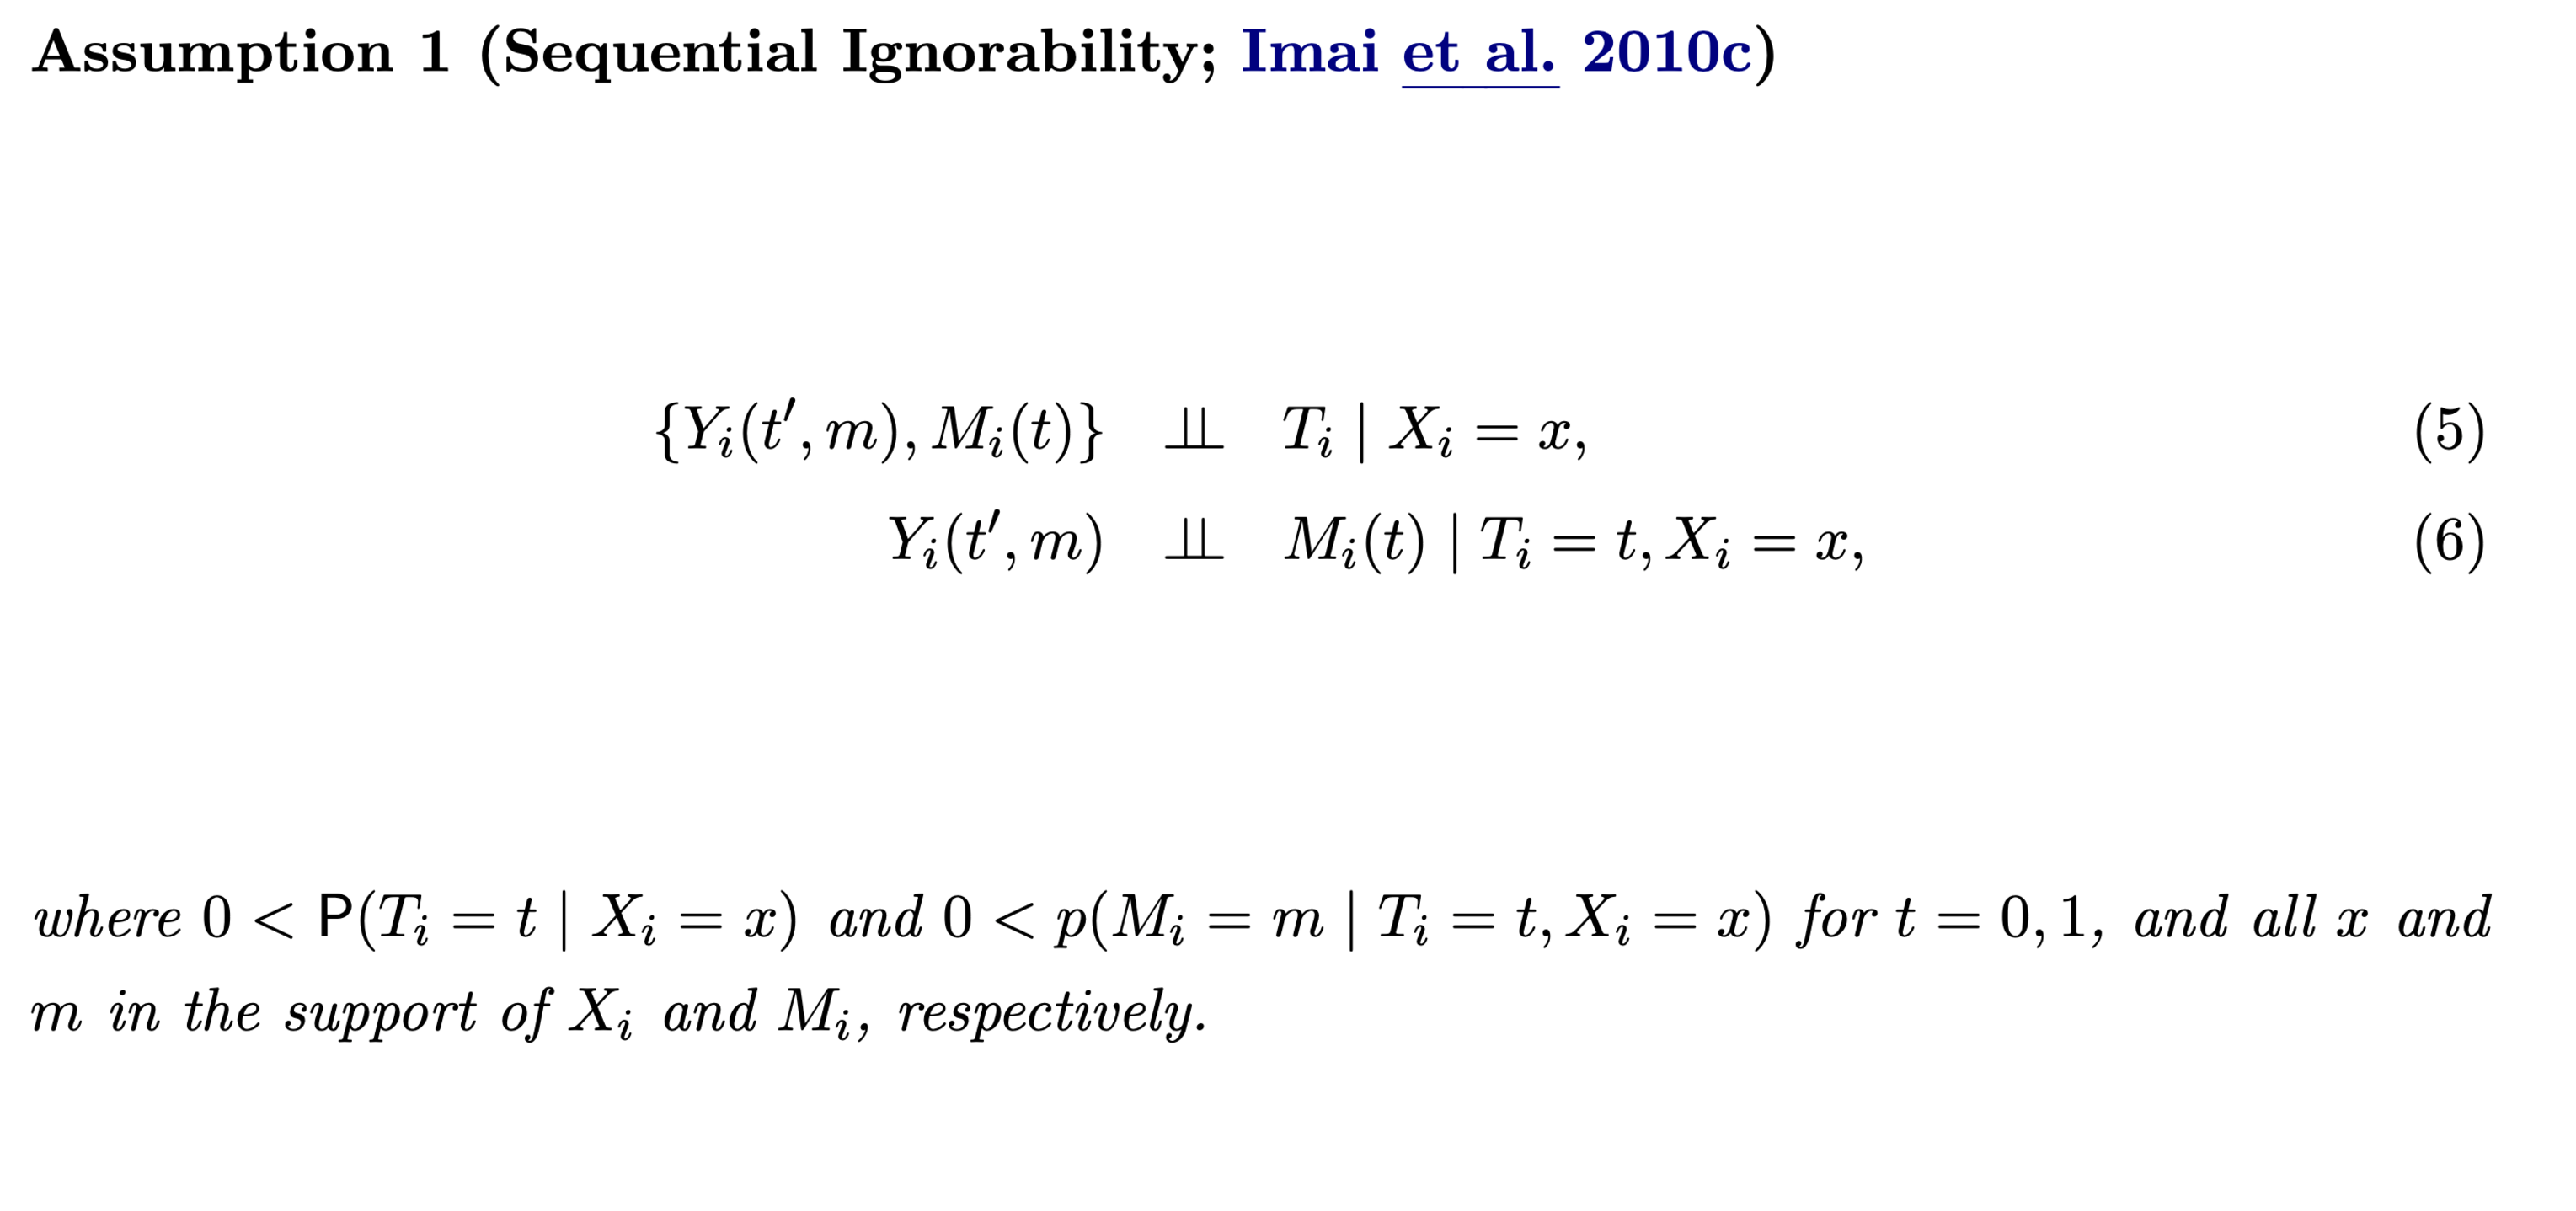
\includegraphics[width=1\textwidth,height=\textheight]{figs/seq}
\end{frame}

\begin{frame}{Estrategias}
\protect\hypertarget{estrategias}{}
\begin{itemize}[<+->]
\tightlist
\item
  Análisis de efectos heterogéneos
\item
  Experimentos paralelos
\item
  Análisis de mediación (Imai y Yamamoto 2013)
\end{itemize}
\end{frame}

\begin{frame}{Análisis de mediación (Imai y Yamamoto 2013)}
\protect\hypertarget{anuxe1lisis-de-mediaciuxf3n-imai-y-yamamoto-2013}{}
\begin{itemize}
\tightlist
\item
  \texttt{Mediation} en R (Tingley et al.~2014)
\item
  Sensibilidad de sus estimaciones a violaciones de la ignorabilidad
  secuencial
\end{itemize}
\end{frame}

\begin{frame}{Análisis de mediación (Imai y Yamamoto 2013)}
\protect\hypertarget{anuxe1lisis-de-mediaciuxf3n-imai-y-yamamoto-2013-1}{}
\center 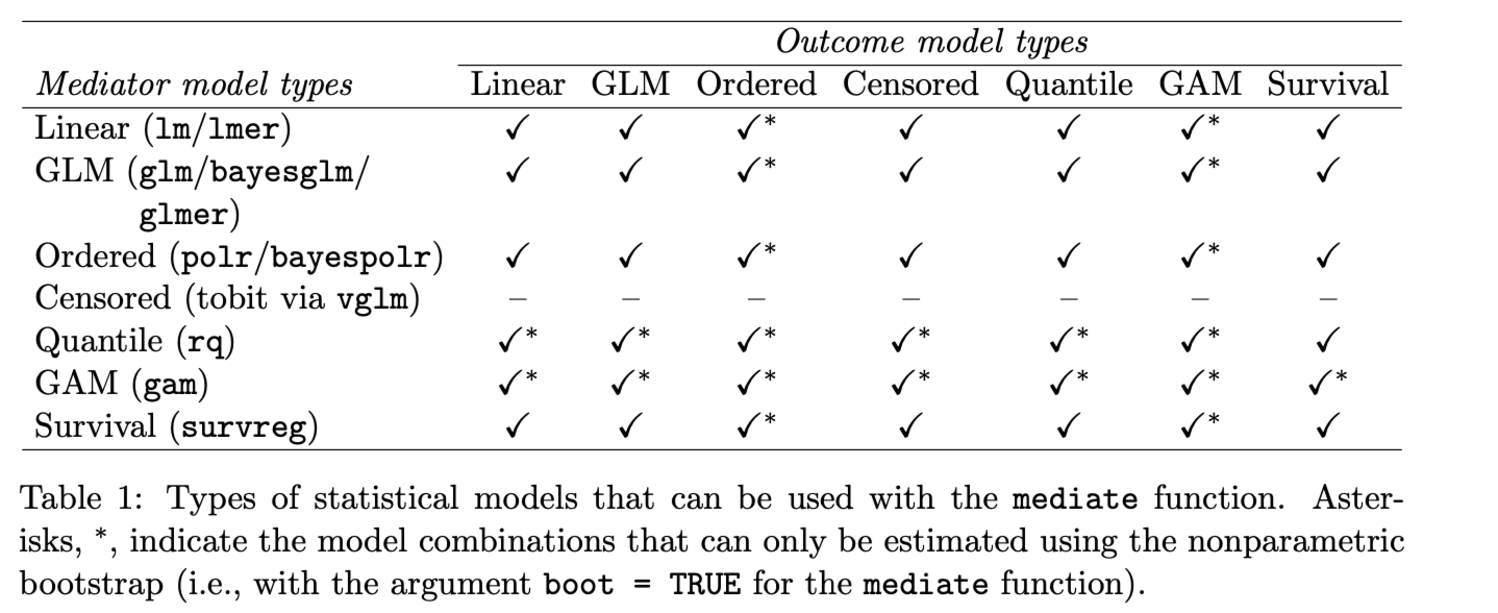
\includegraphics[width=0.8\textwidth,height=\textheight]{figs/models}
\end{frame}

\end{document}
